\documentclass[sigconf]{acmart}


\usepackage{graphicx}
%\usepackage[draft]{graphicx}
\usepackage{subcaption}


\usepackage{booktabs} % For formal tables

\usepackage{bibnames}
\usepackage[T1]{fontenc}
\usepackage{tabularx}

\usepackage{xcolor}
\usepackage{paralist} % for inline lists
%\usepackage[allfiguresdraft]{draftfigure}
\usepackage{hyperref}
\usepackage{multirow}
\usepackage{lipsum}

\usepackage[capitalise,nameinlink]{cleveref}
\def\tightlist{}

\usepackage{import}
\newcommand{\smallunderscore}{\textscale{.5}{\textunderscore}}
\renewcommand{\_}{\textscale{.5}{\textunderscore}}

% Copyright
%\setcopyright{none}
\setcopyright{acmcopyright}
%\setcopyright{acmlicensed}
%\setcopyright{rightsretained}
%\setcopyright{usgov}
%\setcopyright{usgovmixed}
%\setcopyright{cagov}
%\setcopyright{cagovmixed}


% DOI
\acmDOI{xx.xxx/xxx_x}

% ISBN
\acmISBN{979-8-4007-0629-5/25/03}

%Conference
\acmConference[SAC'25]{ACM SAC Conference}{March 31 –April 4, 2025}{Sicily, Italy}
\acmYear{2025}
\copyrightyear{2025}


\acmArticle{4}
\acmPrice{15.00}

% These commands are optional
%\acmBooktitle{Transactions of the ACM Woodstock conference}
%\editor{Jennifer B. Sartor}
%\editor{Theo D'Hondt}
%\editor{Wolfgang De Meuter}


\begin{document}
\title{Evaluation of Uncertainty Estimation in Deep learning using
Constraint-Based Dataset Generation}
%\titlenote{Produces the permission block, and
%  copyright information}
%\subtitle{Extended Abstract}
%\subtitlenote{The full version of the author's guide is available as
%  \texttt{acmart.pdf} document}
  
\renewcommand{\shorttitle}{Uncertainty Evaluation}


\author{Deebul Nair}
%\authornote{Dr.~Trovato insisted his name be first.}
%\orcid{1234-5678-9012}
\affiliation{%
  \institution{SpaceR Research Group }
  \streetaddress{University of Luxembourg}
  %\city{Dublin} 
  %\state{Ohio} 
  \country{Luxembourg}
 % \postcode{43017-6221}  
}
%\email{trovato@corporation.com}

\author{Sathwik Panchangam}
%\authornote{Dr.~Trovato insisted his name be first.}
%\orcid{1234-5678-9012}
\affiliation{%
  \institution{Institute for Artificial Intelligence and Autonomous Systems }
  \streetaddress{Hochschule Bonn-Rhein-Sieg}
  %\city{Dublin} 
  %\state{Ohio} 
  \country{Germany}
 % \postcode{43017-6221}  
}
%\email{trovato@corporation.com}

\author{Miguel A. Olivares-Mendez}
%\authornote{Dr.~Trovato insisted his name be first.}
%\orcid{1234-5678-9012}
\affiliation{%
  \institution{SpaceR Research Group }
  \streetaddress{University of Luxembourg}
  %\city{Dublin} 
  %\state{Ohio} 
  \country{Luxembourg}
 % \postcode{43017-6221}  
}
%\email{trovato@corporation.com}

\author{Nico Hochgeschwender}
%\authornote{Dr.~Trovato insisted his name be first.}
%\orcid{1234-5678-9012}
\affiliation{%
  \institution{ Department of Mathematics and Computer Science }
  \streetaddress{University of Bremen}
  %\city{Dublin} 
  %\state{Ohio} 
  \country{Germany}
 % \postcode{43017-6221}  
}
%\email{trovato@corporation.com}


% The default list of authors is too long for headers}
\renewcommand{\shortauthors}{Nair. D et al.}


\begin{abstract}
{Uncertainty estimation in deep learning methods is a challenging problem
because there is no true label available for uncertainty. Evaluation of the uncertainty estimation
methods is a critical component for determining their practical utility,
particularly when making decisions based on the predictions generated by
a model.}
{This paper identifies the shortcomings of existing techniques for assessing uncertainty estimation methods especially for embodied agent applications. To overcome these limitations, we introduce constraint-based dataset generation.}
{Our methodology allows us to systematically evaluate the performance of
different uncertainty estimation methods in a controlled and
reproducible simulated environment. We generate subset of the datasets for image
classification task based on constraints and then compare the predicted
uncertainties between these subsets based on expert knowledge.}
{We  evaluated three different
uncertainty estimation methods and reported on their differences.}
{The proposed methodology should help in better understanding the uncertainty estimation capability of deep learning models deployed in embodied agents.}

\end{abstract}

%
% The code below should be generated by the tool at
% http://dl.acm.org/ccs.cfm
% Please copy and paste the code instead of the example below. 
%
\begin{CCSXML}
<ccs2012>
   <concept>
       <concept_id>10010520.10010575.10010577</concept_id>
       <concept_desc>Computer systems organization~Reliability</concept_desc>
       <concept_significance>500</concept_significance>
       </concept>
   <concept>
       <concept_id>10010147.10010341.10010342.10010345</concept_id>
       <concept_desc>Computing methodologies~Uncertainty quantification</concept_desc>
       <concept_significance>500</concept_significance>
       </concept>
   <concept>
       <concept_id>10010147.10010257.10010293.10010294</concept_id>
       <concept_desc>Computing methodologies~Neural networks</concept_desc>
       <concept_significance>100</concept_significance>
       </concept>
 </ccs2012>
\end{CCSXML}

\ccsdesc[500]{Computer systems organization~Reliability}
\ccsdesc[500]{Computing methodologies~Uncertainty quantification}
\ccsdesc[100]{Computing methodologies~Neural networks}

\keywords{Uncertainty estimation, synthetic dataset generation, DNN}


\maketitle


\hypertarget{sec:intro}{%
\section{Introduction}\label{sec:intro}}

The accurate estimation of uncertainties in deep learning is a critical
component for deploying them in real-world applications. This has led to
significant interest in developing techniques to estimate uncertainty in
deep neural networks \cite{mena2021survey} \cite{abdar2021review}. For embodied agents like autonomous
car and robots, uncertainty estimation of deep learning models is
particularly important as it can increase the dependability attributes
like safety, reliability, robustness of the embodied agents, enabling
better decision-making in complex environments where uncertainty is
always present. However, evaluating the effectiveness of uncertainty
estimation in deep learning is challenging due to the absence of ground
truth data against which its performance can be measured.

Evaluation of the uncertainty estimation method in the absence of ground
truth is a challenging problem. Uncertainty estimation methods are
evaluated using uncertainty metrics or proper scoring rules \cite{lakshminarayanan2017simple} \cite{gneiting2007strictly},
benchmarking with Bayesian networks outputs \cite{wilson2022evaluating}, reliability
evaluation with out-of-distribution data  \cite{sensoy2018evidential} \cite{kristiadi2021learnable} \cite{kristiadi2020being} and robustness
evaluation with adversarial attack\cite{sensoy2018evidential} \cite{van2020uncertainty} \cite{liu2020simple}  or corrupted data \cite{joppich2022classification} \cite{hendrycks2020augmix}. Even
though these evaluation methods are good metrics for assessing the
effectiveness of uncertainty estimation they are limited in evaluating
only the performance, reliability and robustness. These evaluation
methods fail to evaluate the effectiveness of the uncertainties in the
case of their usage in embodied agents like autonomous car or domestic robots.

Deep neural networks (DNN) have become the de-facto method for perception in robotics due to their exceptional performance with high dimensional data. The output of these networks are utilized to make autonomous decisions for planning and control of the robots. Since the networks are stochastic in nature and also there is noise in sensors we use the probabilistic output of the networks to estimate the state of the environment. These probabilistic outputs are then used as the measurement model in filtering techniques such as the Kalman filter \cite{9746732} \cite{revach2022kalmannet}, Bayes filter \cite{pankert2021deep} or particle filter \cite{karkus2018particle}, which can then be used for state estimation, decision-making under uncertainty and control applications. However, there are no proper evaluation methods to evaluate how the probabilistic outputs of the DNN can be utilized in statistical models, which poses a challenge for real-world applications of DNNs in robotics.
\begin{figure}[t]
	\centering
	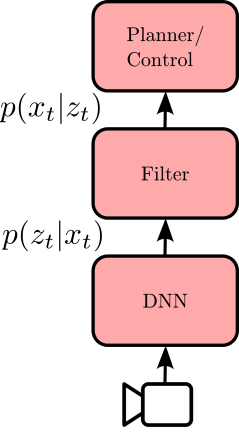
\includegraphics[width=0.25\linewidth]{images/overview}
	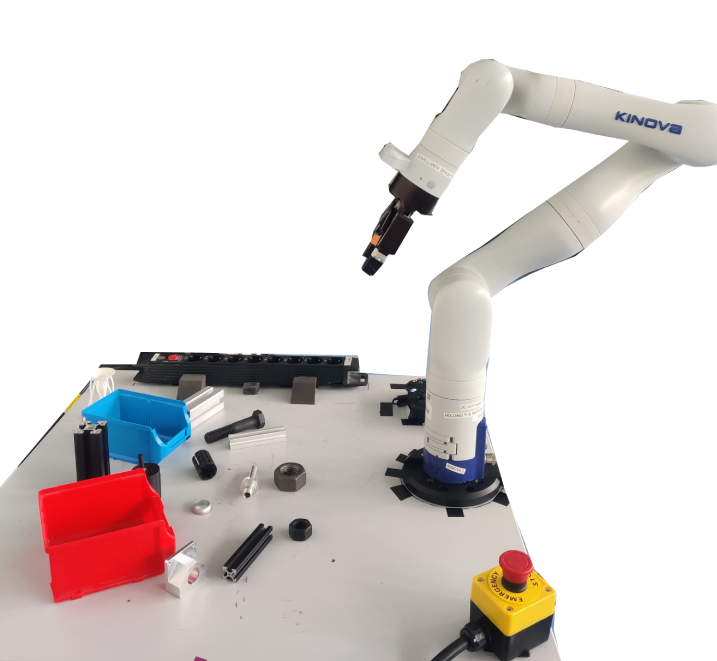
\includegraphics[width=0.60\linewidth]{images/robot_v11}
	%\includegraphics[width=1\linewidth]{images/Constraint_based_dataset_generation_1.png}
	\caption[Overview of usage of uncertainty estimation]{Concept overview of the usage of uncertainty estimation from DNN's in embodied agents for decision making and control. 
	Robot with camera perceiving a scene.}
	\label{fig:overview}
\end{figure}

For example, suppose we are trying to estimate the class of the objects in a cluttered scene using object classification. We use a DNN based classification model to output the probability of objects present on the scene. We can model the relationship between the object classification output and the state of the cup using Bayes theorem. That is, $ p(z_t | x_t) \propto  p(z_t | x_t) p(x_t)$ where $z_t$ is the set of object classification outputs received at time $t$, $x_t$ is the state of the scene at time $t$,  and $p(z_t | x_t)$ is the likelihood of observing the scene given the scene is $x_t$. The likelihood function $p(z_t | x_t)$ may depend on various factors such as the appearance and geometry of the scene, the presence of other objects in the scene, camera angle, environment conditions and the uncertainty estimation capability of the DNN.

To address these limitations, our paper proposes a simulation-based
dataset generation methodology that allows for the systematic evaluation
of uncertainty estimation methods in a controlled and reproducible
environment. We use the heuristics of an expert to determine a set of
constraints that govern the distribution of uncertainties in a simulated
dataset. Based on these parameters we generate a subset of the dataset
which satisfies the specified constraint. The entropy's of the estimated
uncertainty of these datasets generated under constraint are compared
with the entropy's of the nominal dataset. This comparison gives a
better understanding on how the uncertainty behaves in different
scenarios the embodies agent perceives in the real world. Examples of
constraints are distance of object from the camera, lightning condition
of the environment, texture of the environment, deformability of the
objects etc. 
%Consider the constraint of distance of objects, the expected behaviour will be when the object is far from the camera the uncertainty should be high as compared to the uncertainty of objectswhich are near to the camera. Based on this constraint we generate 2 subset of datasets  called far\_dataset and near\_dataset. Now we record the uncertainty estimated by different uncertainty estimation methods and then we verify how our assumption .

The contributions of the work are : 
\begin{inparaenum}[\itshape a\upshape)]
	\item We identify the limitations of
	current evaluation methods for deep learning models used in embodied
	agents (machines that interact with their environment).
	\item We propose a
	new method to generate datasets for evaluating these models using
	Blender, a 3D graphics software.
	\item  We use these generated datasets to test and
	compare the performance of different uncertainty estimation methods for
	these models.
\end{inparaenum}

%\import{./}{limitation}


\hypertarget{limitation-of-evaluation-methods-of-uncertainty-estimation-of-dnn}{%
\section{Limitation of evaluation methods of uncertainty estimation of
DNN}\label{limitation-of-evaluation-methods-of-uncertainty-estimation-of-dnn}}

In this section we discuss the different methods used to evaluate uncertainty estimation methods and their limitations with respect to their usage in embodied agents.

\hypertarget{uncertainty-metric-based-evaluation}{%
\subsection{Uncertainty metric based evaluation}
\label{uncertainty-metric-based-evaluation}}

The most common method for evaluating uncertainties is by using the
different uncertainty metrics. The most commonly used metrics for
discrete outputs are Brier score \cite{gal2016dropout} \cite{lakshminarayanan2017simple} \cite{liu2020simple}, expected calibration
error \cite{carneiro2020deep} \cite{maddox2019simple}, negative log-likelihood and  \cite{loquercio2020general} \cite{wang2019deep} \cite{sensoy2018evidential}. Even though these metrics provide a
quantitative measure of the estimated uncertainty, they fail to capture
the entire range of possible outcomes and can be biased by model performance. The Brier score has the drawback of being
influenced by the number of categories in the dataset \cite{assel2017brier}  . In
multi-class classification tasks, the Brier score may be biased towards
models that predict a larger number of classes, even if their
predictions are less accurate \cite{rindt2022survival}. This can make it difficult to compare
models with different numbers of classes. In case of
expected calibration error the result depends upon the distribution of
data across the number of bins used for calculation and the number of
bins chosen affects the ECE algorithm  \cite{nixon2019measuring}. This means that
models with low ECE can still have poorly calibrated predictions or be
overconfident in its predictions. Negative log likelihood gives more
preference to the correctness of the output than to the uncertainty
correctness \cite{Ashukha2020PitfallsOI}. We still
can use these metrics to evaluate the performance, in this work we use entropy as
a measurement of the uncertainty and use it to compare dataset
subsets.

\hypertarget{robustness-evaluation-with-adversarial-attack-and-corrupted-dataset}{%
\subsection{Robustness evaluation with adversarial and corrupted data}\label{robustness-evaluation-with-adversarial-attack-and-corrupted-dataset}}

Another avenue for evaluating uncertainty estimation is by assessing the
robustness of the DNN to adversarial attacks \cite{sensoy2018evidential} \cite{van2020uncertainty} \cite{liu2020simple}  and corrupted datasets  \cite{joppich2022classification} \cite{hendrycks2020augmix}. The expected behavior is that the
uncertainty estimate of the adversarial attack dataset and the corrupted
dataset is higher than the original, clean dataset. This is an example
of using the heuristics of experts to evaluate uncertainty estimates. We
expand on this idea by generating multiple subsets of clean and corrupted datasets
which the embodied agent can see over its lifetime and use them as
testing datasets.

\hypertarget{reliability-evaluation-with-ood-dataset}{%
\subsection{Reliability evaluation with Out-of-Distribution (OOD) dataset}\label{reliability-evaluation-with-ood-dataset}}

In addition to robustness evaluation, reliability evaluation with
out-of-distribution datasets is another important aspect of the
evaluation of uncertainty estimation \cite{sensoy2018evidential} \cite{kristiadi2021learnable} \cite{kristiadi2020being}. In
this evaluation, the expected outcome is that the uncertainty estimate
of the OOD dataset is higher than that of the in-distribution dataset.
This is also a valid assumption and is also an example of using expert
heuristics to evaluate uncertainty estimates. We argue that for the
reliability test not only out-of-distribution we also have to look into
different subsets of in-distribution and verify the change of
uncertainty.






\begin{figure*}[t]
	\centering
	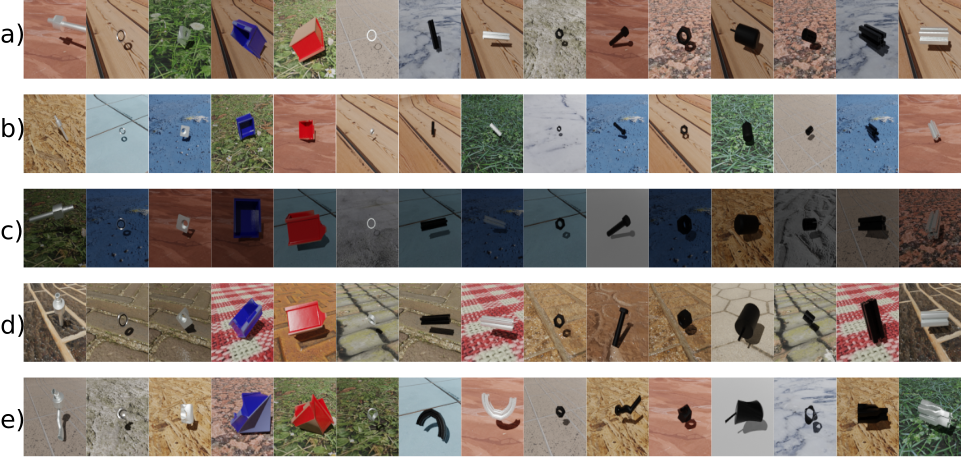
\includegraphics[width = \textwidth]{images/dataset_generation_v3.png}
	\caption{Dataset generated with Blender under specific constraints a) Normal b) Far c) Dark d) Texture e) Deformed}
	\label{fig:constraint_based_dataset_generation}
\end{figure*}


\hypertarget{constraint-based-subset-dataset-generation-using-blender}{%
\section{Constraint based subset dataset generation using
Blender}\label{constraint-based-subset-dataset-generation-using-blender}}

We take inspiration from software testing and verification,
where the human expert provides expected input and output to generate test cases
that certify the performance of the software under various possible inputs. We expand on
this idea to test uncertainty estimates of DNN's by generating
constraint-based datasets that cover different scenarios that the DNN is
expected to encounter during its operation. However, since the expected
true uncertainty is not a quantifiable value it difficult for humans to
provide the true expected uncertainty. However, humans are good with
provided comparative judgments between uncertain situations, allowing us
to generate pairs of datasets with varying degrees of uncertainty. For
example, the uncertainty of objects which are far away from the camera
is expected to be higher than objects nearer to it. We use simulation
based dataset generator as it allows us to control various factors such
as lighting conditions, object occlusion, and camera angle while
generating datasets with varying degrees of uncertainty.


%In real world, the embodied agent has to perceive the environment to make a decision. The environment has many variations like lighting, occlusion and scenarios where the images are blurry or the perceiving environment itself changes. For a deep learning model it is very much required to represent the uncertainty reliably in such scenarios to avoid failures and catastrophes. To represent the uncertainty in such scenarios the deep learning models must be evaluated on the datasets representing such scenarios. Collecting datasets for different real world scenarios is however not a suitable option because of the limitiations of time and cost. But all these scenarios can be simulated in a graphics software like blender and corresponding synthetic datasets can be generated.\\


In this methodology, we try to leverage the Blender software to create simulation based synthetic datasets. Blender \cite{Blender}  is a free and open-source 3D creation software used for creating 3D models, animations, and visual effects. Its features such as modeling, texturing, and rendering make it a powerful tool for creating realistic 3D environments and objects. It is used to develop dataset for training deep learning models \cite{Denninger2023}. Blender's ability to automate and randomize certain aspects of the dataset generation process makes it particularly useful for training deep learning models that require large and diverse datasets. We begin our approach by enumerating the heuristics for a specific constraint from a deep learning expert. The defined heuristics are used to identify a set of modifiable  parameters in blender which are used to generate a nominal dataset and a subset of dataset which satisfies the specific constraint. 
%Next we need the CAD models for the objects that are being perceived by the agent in the real world. These objects can either be designed by the user in the blender software itself or they can be imported from open sources libraries like ShapeNet \cite{shapenet2015} along with the object's textures. 
In order to generate the datasets we need an environment, for this we create a scene in blender which consists of different components like, a background plane, a camera and a light source. By changing the parameters of these components such as intensity of light, focal length of camera, texture of background plane etc, we introduce variations to the datasets based on the heuristics defined by the expert. 
%We have a configuration file for the modifiable parameters in blender. Using this configuration and the scene that we have created before, we import the cad models into the scene and render the images under different conditions. 
We create a nominal dataset with all variations of the environment and different subset of datasets which satisfy particular constraints. In the nominal dataset all the objects present in the scene appear in normal conditions and there is all the variations introduced to the environment. On the other hand, for each subset of datasets we fix a particular variation and only generate those dataset which satisfies the constraint. For our experiments we generated  4 variations based on distance of object, lighting condition, background texture and deformation of objects.
We selected a set of texture less industrial objects with 16 classes. All the objects had CAD models available which was the criteria for their selection. 
%of lighting to create bright\_lighting, dark\_lighting datasets, for the distance constraint we introduce variation in the focal length parameter of the camera to create far\_distance, near\_distance datasets, Also we use the depth of field parameter of the camera to create blur constraint dataset. By changing the textures of the background plane we introduce a constraint for the textures and by using the modifiers present in the blender software we deform the shape of the object to create a deformation constraint. Finally, the generated nominal dataset is used for training of different deep learning models and the subsets of constriant datasets are used for evaluating the performance of the trained models based on entropy comparison.

\begin{table*}[b]
	\centering
\begin{tabularx}{\textwidth} { 
	|>{\hsize=.20\hsize}X
	|| >{\hsize=.80\hsize}X| }
	\hline
	\textbf{Constraint}  & \textbf{Hypothesis} \\
	\hline
	Distance  & The uncertainty of objects far from camera  \textbf{shall} be higher than objects at nominal distance. \\
	\hline
	Lighting  & The uncertainty of objects in dark lighting  \textbf{shall} be higher than nominal lighting condition. \\
	\hline
	Texture & The uncertainty of objects on textured surface \textbf{shall} be same as uncertainty with plane surface. \\
	\hline 
	Deformation & The uncertainty of objects with deformation \textbf{shall} be higher than nominal objects. \\
	\hline
\end{tabularx}
 \caption{Constraint dataset types and the expected uncertainty in those dataset}
\label{table:constraints_table}
\end{table*}
\hypertarget{experiments}{%
\section{Experiments}\label{experiments}}

  In this work, we have selected four uncertainty estimation methods: cross-entropy model, MC dropout model \cite{gal2016dropout}, evidential deep learning model \cite{sensoy2018evidential} and ensembles model \cite{lakshminarayanan2017simple}. We used ResNet18 architecture for the cross-entropy, dropout and evidential models and for the ensembles model we have averaged the results of four deep learning models. For training the four models we have used PyTorch framework keeping the hyper-parameters same for all the models. For all the experiments we used the step learning rate scheduler with a learning rate of 0.001. We have chosen the batch size as 128 and a weight decay of 1e5. In the following experiments all the four models are trained with normal dataset 
 \ref{fig:constraint_based_dataset_generation} and their performance is tested with the constraint datasets. For comparing and evaluating the expected behavior of the uncertainty estimation methods we compare the box plot of the entropy of the dataset. 
 %In the following experiments we expect the uncertainty of test constraints to be greater than the uncertainty of training constraint. Also, for a good uncertainty estimation method it is expected that the entropy of incorrect predictions to be high. This implies that there is no high confidence values being assigned for the miss classifications. Thus from the following experiments, in the boxplots we expect to observe a clear separation between the entropy of correct and incorrect predictions.

\subsection{RQ1: Do predicted uncertainties change based on object distance?}

To evaluate the performance of uncertainty estimation methods in the scenario of distance of object to camera, we have created two constraints far and near. The hypothesis for the impact of object's distance condition is that when the models trained on normal conditions and tested with the far distance dataset we expect the uncertainty to be high. To check this hypothesis, we have trained four uncertainty estimation methods on normal conditions dataset and test their performance on far constraint dataset. The entropy of both the dataset is plotted in \cref{fig:entropy_far}
%, in the case of cross-entropy, dropout and ensembles models, we can see that there is no separation for the entropy of correct and incorrect predictions of far distance constraint. Also, for the incorrect predictions these three models have low entropy values implying that the models are providing high confidence to the miss-classifications and thus their outputs cannot be trusted. 
%On the other hand even-though 45\% of the incorrect predictions of far constraint lie in the region of correct predictions of far constraint, the separation is high when compared to other three models. Hence when compared to other other three model, the performance of evidential is good in far distance constraint. Also, from the table \ref{tab:accuracy_table}, for both far and near constraints, we can see that the accuracy of all the four models is very low. This represents that the models are not able to generalize the distance of objects.
We observe that the the entropy for correctly classified (orange bar) predictions for all uncertainty estimation methods is higher than the near dataset. This confirms that the models learn make changes to the uncertainty based on the distance. We also observe the entropy range of correctly classified far dataset is very much near to entropy of miss-classifed (red bar) for cross-entropy, dropout and ensembles method, while there is highest separation for the evidential loss function. This is of particular importance because based on the entropy of the miss-classified classes different decision making algorithms are written.

\begin{figure*}[t]
	\centering
	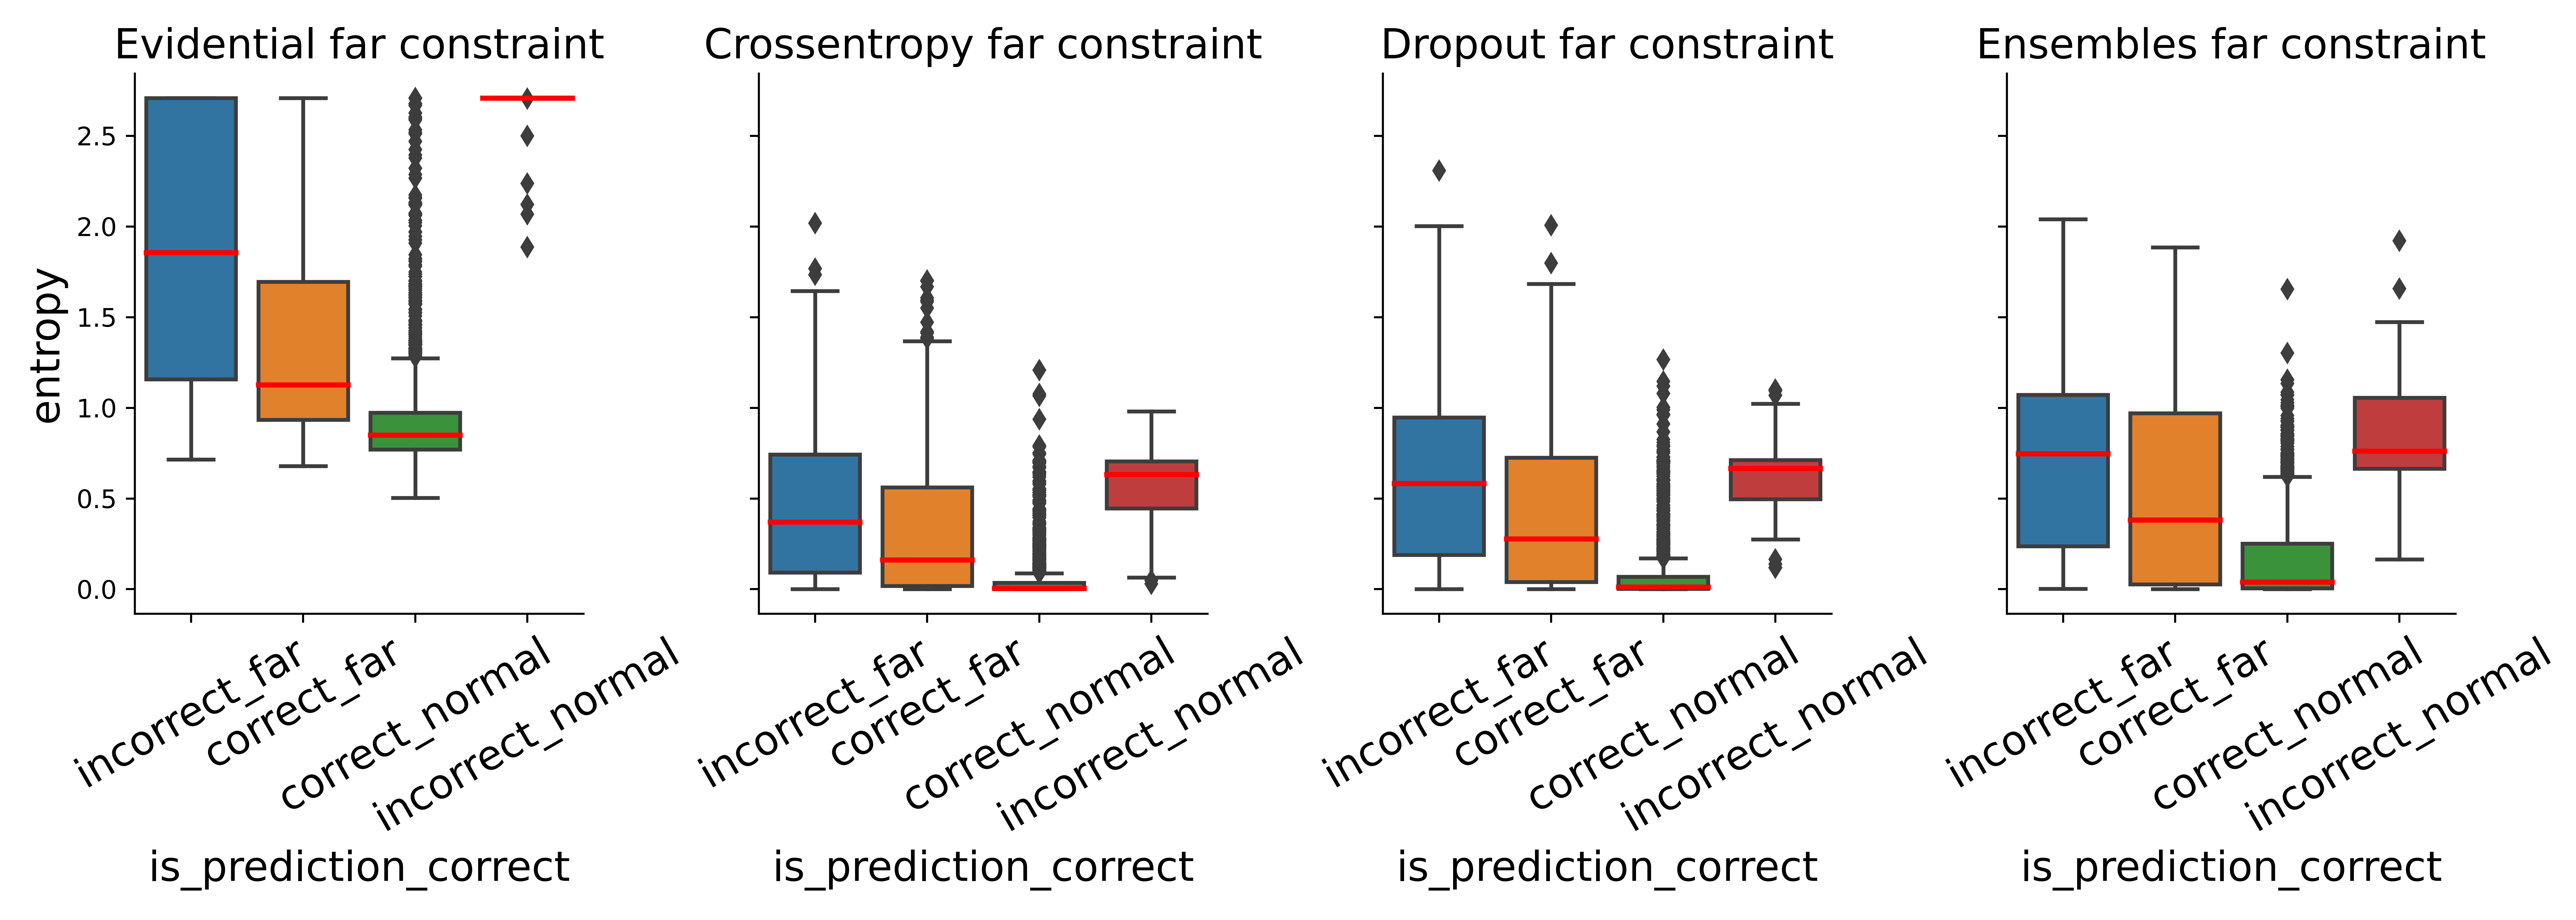
\includegraphics[width=\textwidth]{images/entropy_far_constraint.png}
	\caption{Entropy comparison of uncertainty estimation methods for nominal and far distance dataset.}
	\label{fig:entropy_far}
\end{figure*}

%In the case of near distance constraint, from the figure \ref{fig:entropy_near}, we can observe that there is a clear separation between correct and incorrect predictions of near constraint in the case of evidential model alone. Hence we consider the performance of evidential model to be good when compared to crossentropy, dropout and ensembles models. Also, we can see that both crossentropy and dropout models have high confidence values for the miss-classifications and thus the outputs from these two models cannot be trusted in the case of near distance constraint.

%\begin{figure}[t]
%	\centering
%	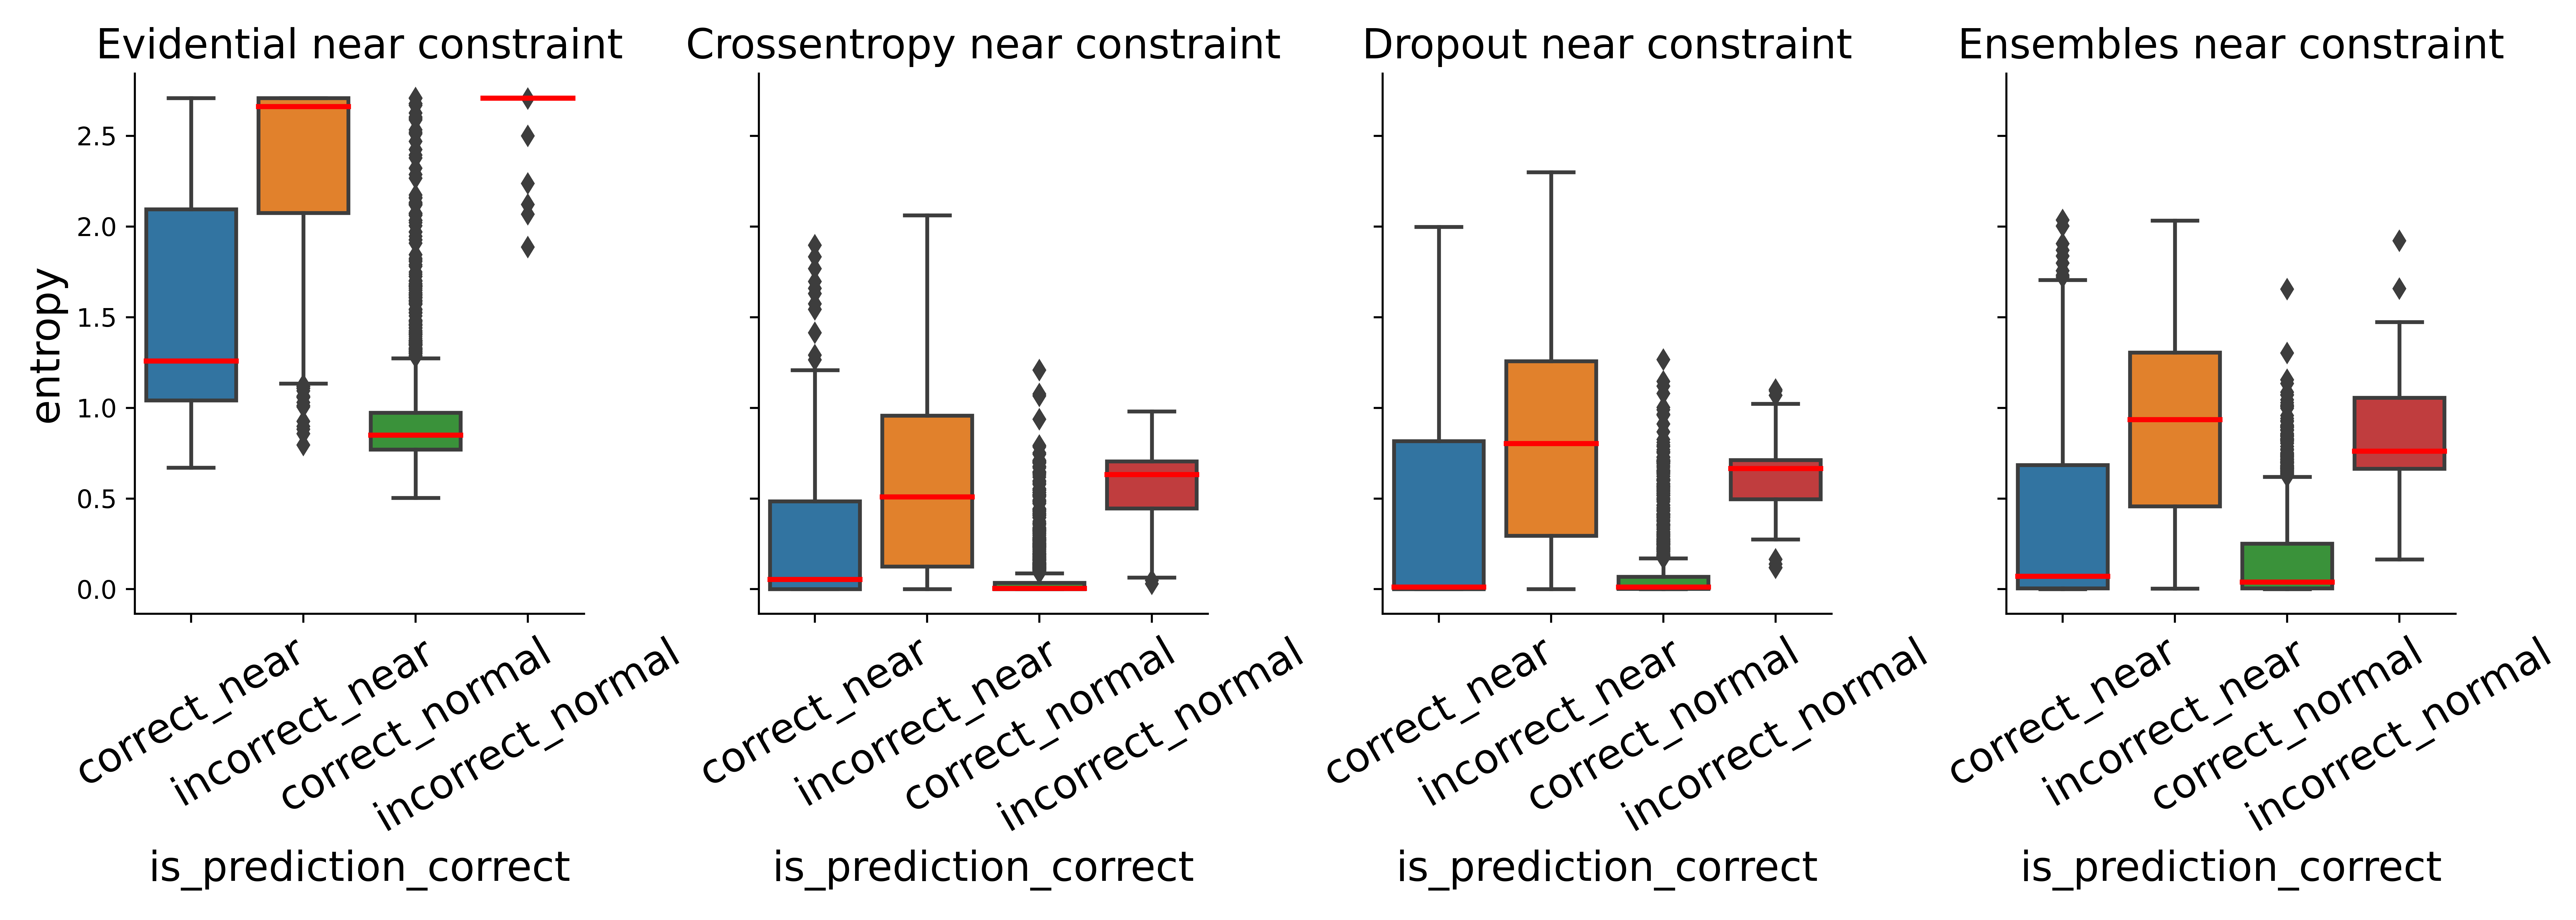
\includegraphics[width=\textwidth]{images/entropy_near_constraint.png}
%	\caption{Entropy near distance constraint}
%	\label{fig:entropy_near}
%\end{figure}

\subsection{RQ2: Do predicted uncertainty change when lightning change?}

\begin{figure*}[b]
	\centering
	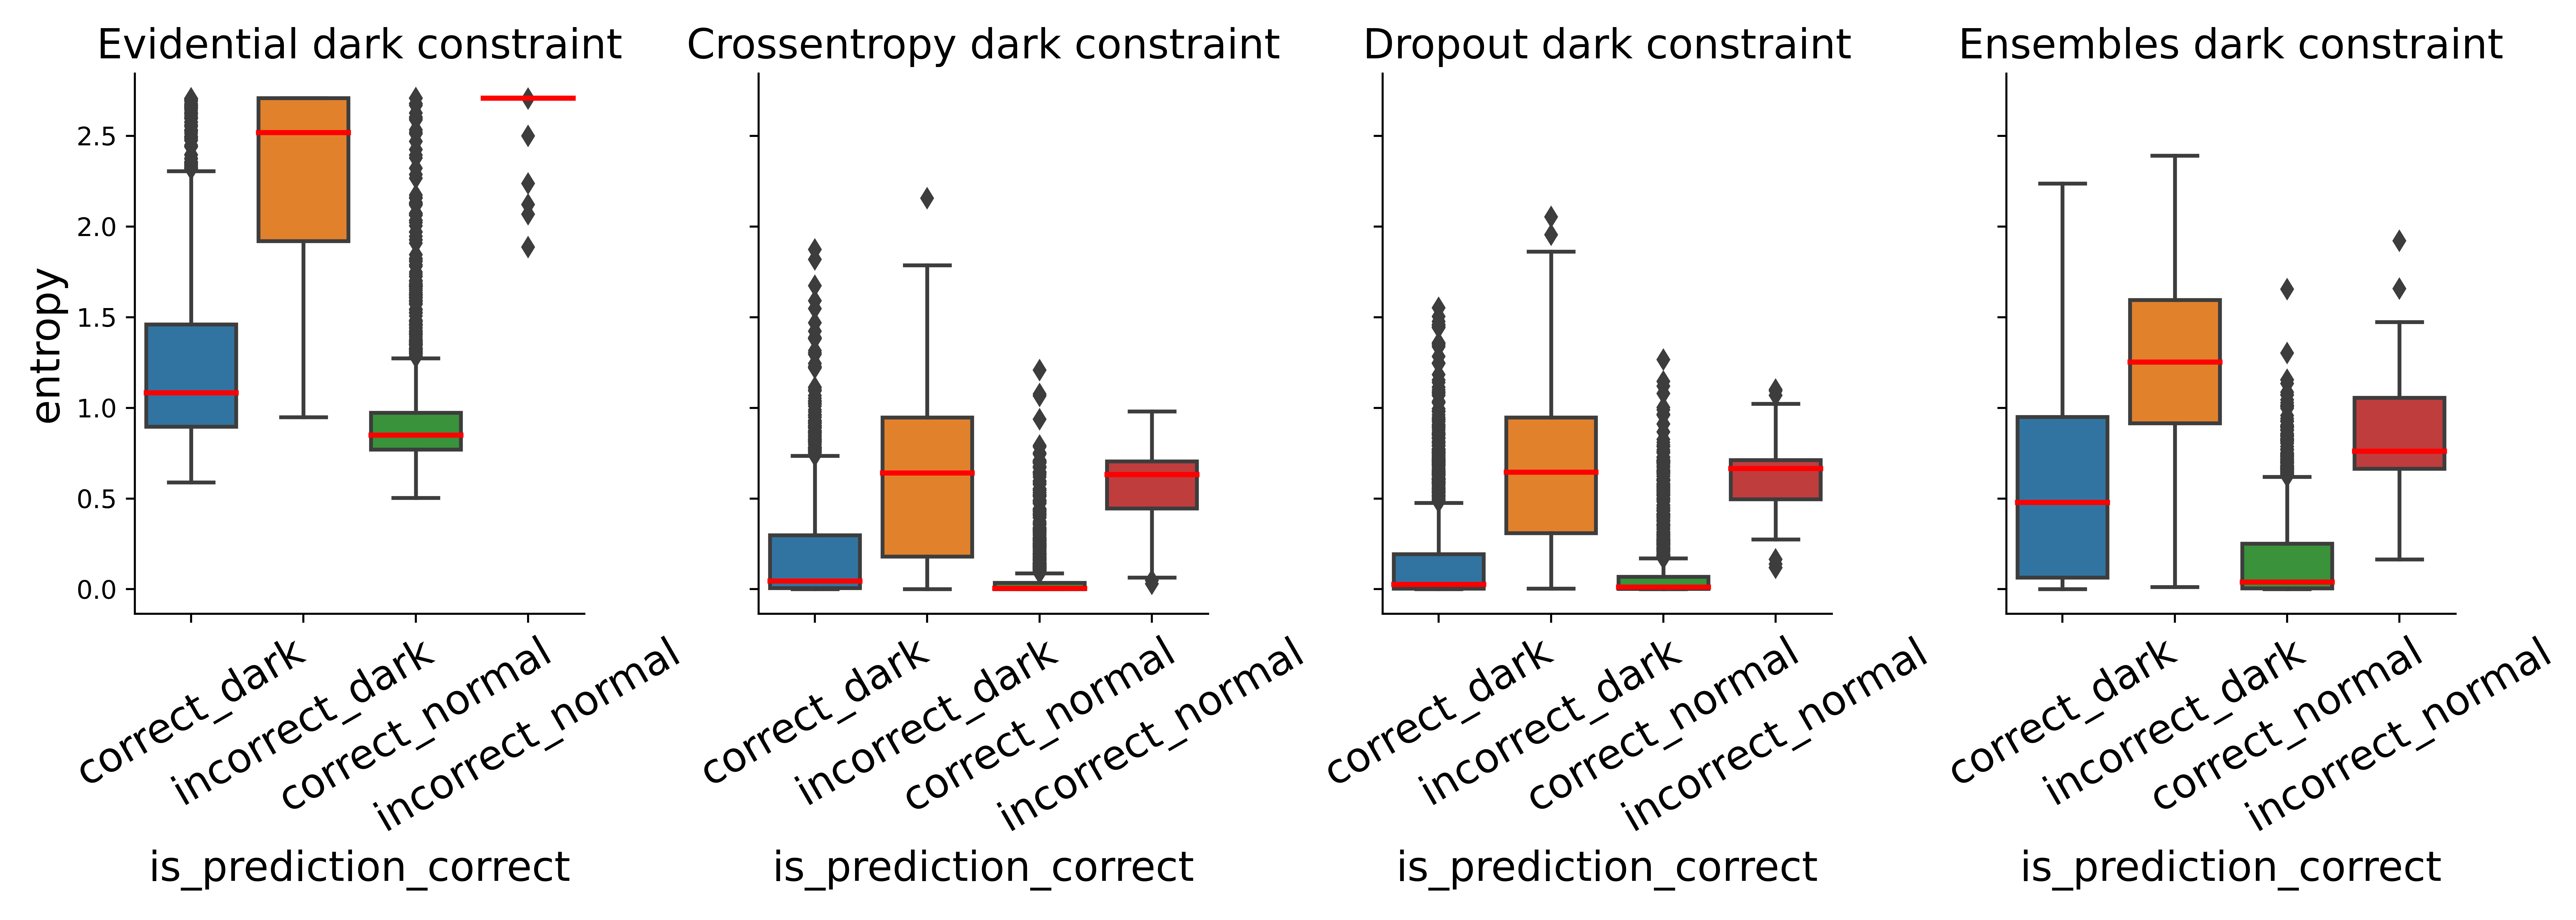
\includegraphics[width=\textwidth]{images/entropy_dark_constraint.png}
	\caption{Entropy comparison of uncertainty estimation methods for nominal and dark lighting dataset.}
	\label{fig:entropy_dark}
\end{figure*}


To evaluate the performance of the uncertainty estimation methods on environmental lighting conditions, we have created the dark constraint dataset. The hypothesis for the impact of lighting conditions is that when the models trained on normal conditions and tested with dark lighting dataset,  we expect the uncertainty to be high in the dark dataset. The entropy of both the dataset are plotted in \cref{fig:entropy_dark}. 
%For the bright constraint from the figure \ref{fig:entropy_bright}, we can see that in the case of crossentropy loss and dropout models there is no increase in uncertainty and also they have low entropy values for the incorrect predictions. This shows that both crossentropy loss and dropout models are providing high confidence values to the miss-classifications and thus they are not reliable. But in the case of evidential and ensembles models, we can clearly see there is a differentiation between the entropy of correct and incorrect predictions. This shows that both evidential and ensemble models are not providing high confidence values to the miss-classifications and thus the predictions of these two models can be trusted. On the overall because of the properties of evidential loss and dirichlet distribution we can see a maximum separation between the correct and incorrect predictions of bright constraint. Thus the performance of evidenital model is good when compared to other three models.

%\begin{figure}[t]
%    \centering
%    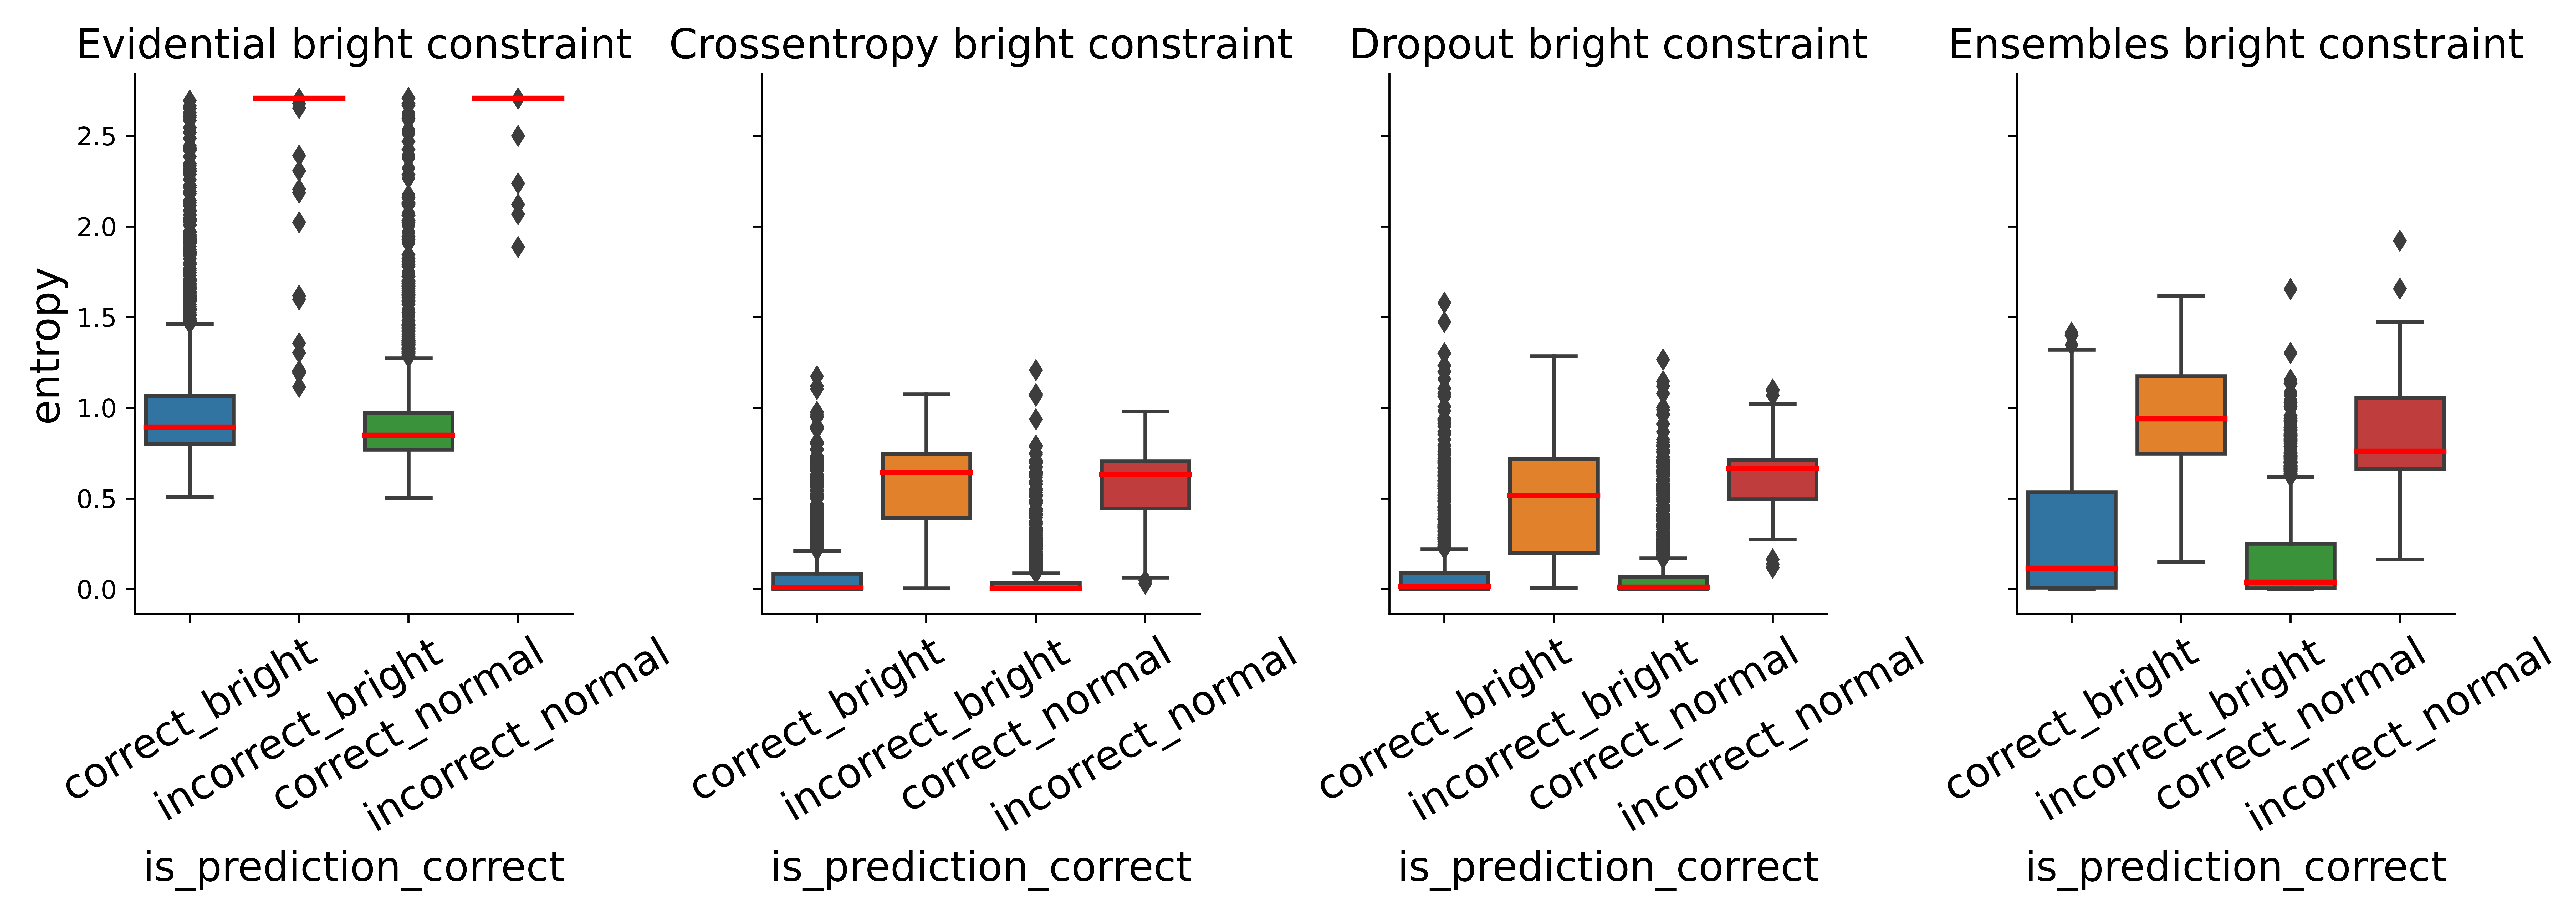
\includegraphics[width=\textwidth]{images/entropy_bright_constraint.png}
%    \caption{Entropy bright lighting constraint}
%    \label{fig:entropy_bright}
%\end{figure}

%For the case of dark lighting constraint the predicted entropy value are plotted in figure \ref{fig:entropy_dark}. Both cross-entropy and dropout models have high confidence values for the miss-classifications, so the outputs from these two models cannot be trusted. In the case of evidential and Ensembles models we can see a clear separation between the entropy of correct and incorrect predictions. This shows that both evidential and ensemble models are not providing high confidence values to the miss-classifications and thus the outputs from these models can be trusted. As again, since the maximum separation for the entropy is seen in evidential model we consider it as the good performing method. Also, from the table \ref{tab:accuracy_table}, we can see that the accuracy of all the four models in dark constraint is very less implying that the models are not able to generalize on the dark constraint.
We observe that our hypothesis is accepted for all the 4 methods. The entropy of the dark dataset is higher than the normal dataset. We also observe there is entropy of the correct predictions in the dark dataset is separated from the incorrect of the normal dataset. 


\subsection{RQ3: Do predicted uncertainty change when the background change?}
To evaluate the performance of uncertainty estimation methods in the scenario of change in background textures, we have created a constraint dataset called textures. The image backgrounds present in textures dataset does not belong to the image backgrounds present in normal conditions dataset, thereby ensuring that the images present in textures constraint are not seen during the training process. The hypothesis for the impact of environmental background conditions is, when the models trained on normal conditions are tested with the images present in textures constraint we expect the uncertainty to be same as the model has never seen such textures before, as we are learning the object and not the background. To check this hypothesis, we have trained four uncertainty estimation methods on normal conditions dataset and test their performance on textures constraint dataset. From the figure\cref{fig:entropy_textures}, 
%For evidential model, we can see that there is an overlap for the entropy of correct and incorrect predictions and thus its performance is poor in textures constraint. In the case of cross entropy and dropout model, even though there a separation of the entropy of correct and incorrect predictions, the entropy of incorrect predictions is low implying that these two models are providing high confidence values to the miss classifications. Hence the output of these two models cannot be trusted. On the other hand, for ensembles model, we see a clear separation between the entropy of correct and incorrect predictions. Thus in the case of textures constraint, we consider the performance of ensembles model to be better when compared to evidential, cross-entropy and dropout models. 
%Also, from the table \ref{tab:accuracy_table}, we can see that the accuracy of ensemble models is high in the case of textures constraint and results from the entropy are also same. 
Based on the observations we can accept the hypothesis for all the constraints. We observe there is minimal change of entropy for correct predictions when the background changes.  We also observe ensemble has the highest change in entropy indicating ensembles also learn about the background.
 
\begin{figure*}[t]
    \centering
    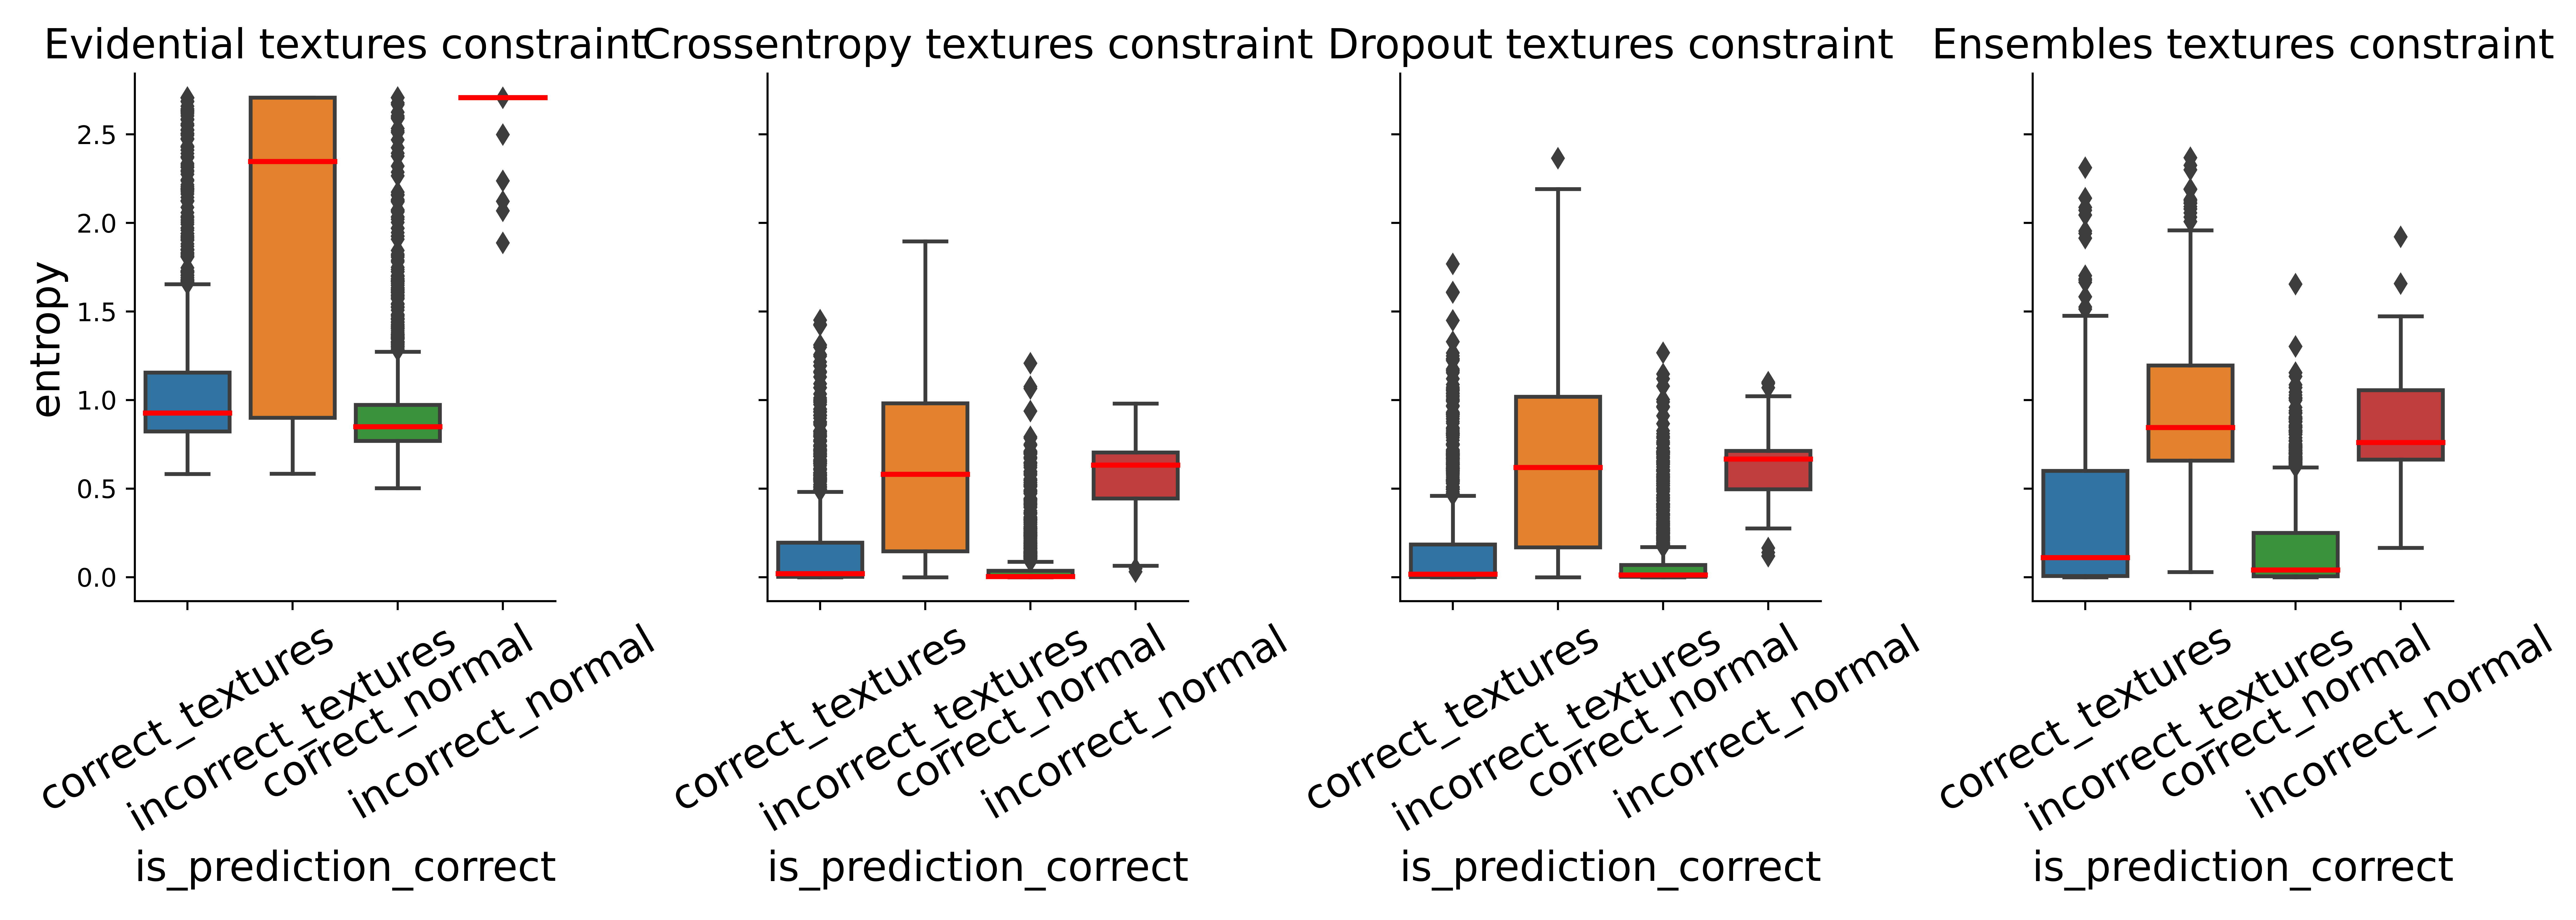
\includegraphics[width=\textwidth]{images/entropy_textures_constraint.png}
    \caption{Entropy comparison of uncertainty estimation methods for nominal and texture dataset.}
    \label{fig:entropy_textures}
\end{figure*}

\subsection{RQ4: Do predicted uncertainty change when object's shape is deformed? }

To evaluate the performance of uncertainty estimation methods in the scenario of change in the object's shape, we have created a constraint called deformation. In this experiment we have generated a normal data set  in which all the objects are in proper shape and used it for training. For the test case we have deformed the shape of the objects such that it is possible and seen in the real world scenarios. Using these deformed objects we have generated test data for deformation constraint. The hypothesis for the impact of object's deformation constraint is, that we expect some uncertaintyto increase in the deformed dataset. From the figure \ref{fig:entropy_deformation}.
% we can see that in the case of evidential model alone a clear difference between the entropy of correct and incorrect predictions is observed. In the case of crossentropy, dropout and ensembles models, the separation is minimum and also, we can see that the entropy of incorrect predictions of deformation constraint is low. This implies that crossentropy, dropout and ensembles models are providing high confidence values for the miss-classifications and thus their outputs cannot be trusted. 
We have to reject his hypothesis as you can see that when the objects are deformed there is very minimal change in entropy of the correct classified objects. This indicates that the uncertainty estimation methods are not sensitive to the objects shape.
%Also, from the table \ref{tab:accuracy_table}, we can see that the accuracy of evidential model is high when compared to other three models, but all the three models, cross-entropy, dropout and ensemble models also have high accuracy. Based on the entropy results we found that these three models are assigning high confidence values to the incorrect predictions and thus the outputs from them cannot be trusted. From this we can say that relying on accuracy metric alone is not sufficient for comparing the performance of uncertainty estimation methods.

\begin{figure*}[t]
    \centering
    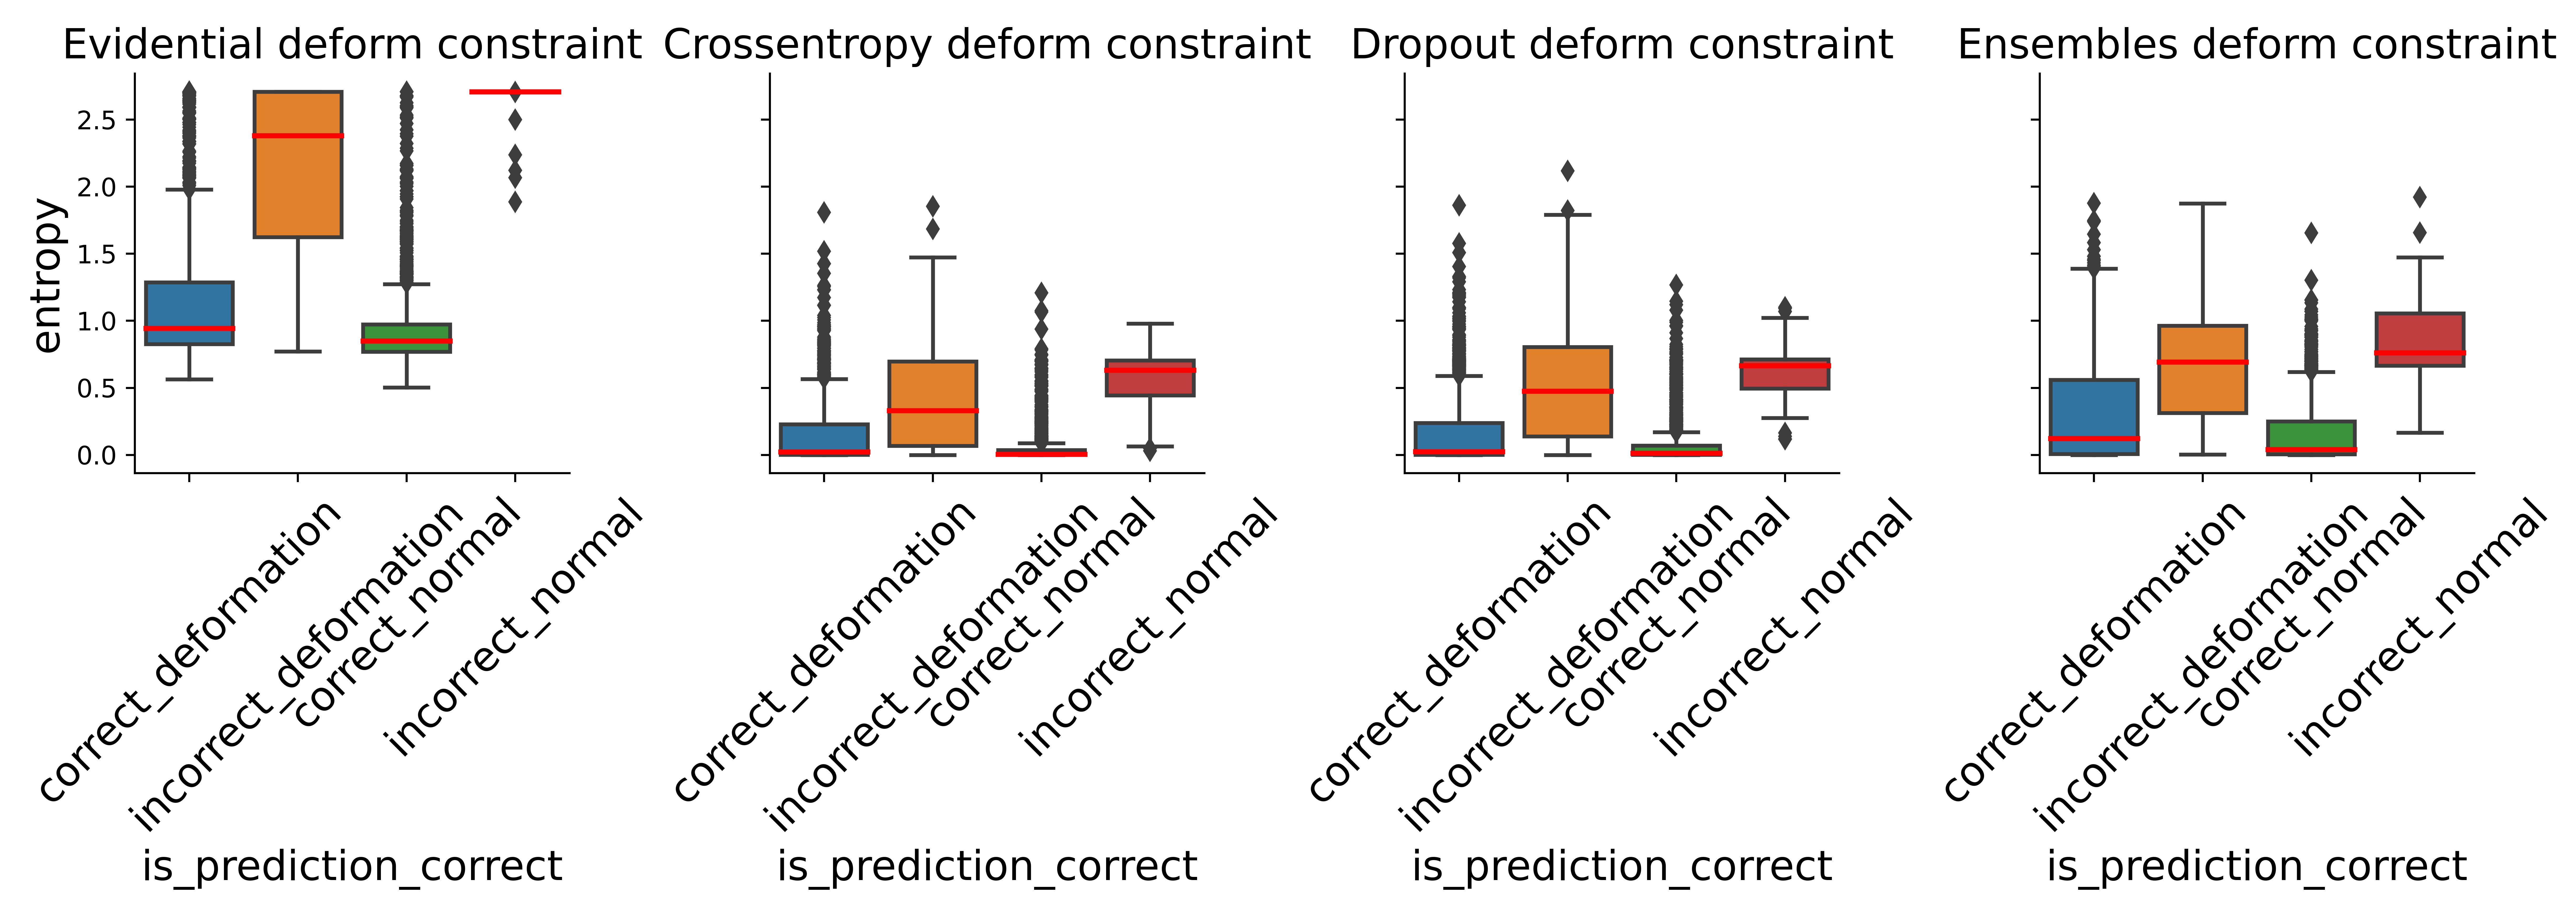
\includegraphics[width=\textwidth]{images/entropy_deformation_constraint.png}
    \caption{Entropy comparison of uncertainty estimation methods for nominal and deformed dataset.}
    \label{fig:entropy_deformation}
\end{figure*}



\hypertarget{discussions}{%
\section{Discussions}\label{discussions}}
The advantage of the proposed methodology is that one can generate any new subset of the dataset based on a any new constraint. As uncertainty cannot be measured one can only evaluate the methods based on heuristics of human experts. The methodology enables such experts to develop test dataset and complete the evaluation. DNN's developed for perception of environments in embodied agents requires additional evaluation methods as compared to fixed environment tasks like medical diagnosis datasets.  One limitation of the methodology is that one has to generate the scenes in Blender which are similar to real world scenes. We have open sourced the dataset generation code here \url{https://github.com/DependableSoftware2-0/ConstraintBasedBlenderDatasetGenerator}. Future work we would like to add additional constraints to the dataset generator.

\hypertarget{conclusions}{%
\section{Conclusions}\label{conclusions}}
Uncertainty estimates from the deep learning networks are used as observation models in different statistical models like filtering, state estimation and decision under uncertainty. The current evaluation methods focus majorly on robustness and reliability attributes but fail to evaluate their performance as required by statistical models. In this work, we focussed on addressing this gap and proposed an artificially generated dataset based on constraints to test the uncertainty estimates of deep neural networks.
The proposed method generates this subset of a dataset based on a particular scenario that the DNN will observe when its deployed. For each subset, a human expert  provided the expected uncertainty estimate behavior.  The predicted and expected uncertainties are utilized to evaluate the performance of the DNN.
We compared 3 state-of-art uncertainty estimation methods for the task of object classification of non-texture industrial objects. We trained the models using the dataset generated and for evaluating the uncertainties we generated 3 constraint-based dataset based on distance, lightning condition, background and deformation. 
For each constraint dataset, we mentioned the expected uncertainty and then used the entropy of the predictions to compare with the hypothesis.
Based on our hypothesis we learned that the uncertainty estimation methods learn about lightning conditions and object distance to camera however the methods dont learn about the shape of objects.
We hope the proposed methodology helps in a better understanding of uncertainty estimation methods.


\section{Acknowledgments}
Deebul Nair gratefully acknowledges the ongoing support
of the Bonn-Aachen International Center for Information Technology and a PhD
scholarship from the Graduate Institute of the Bonn-Rhein-Sieg University. This
work was supported by the European Union’s Horizon 2020 project SESAME (grant agreement No 101017258).


\begin{acks}
  The authors would like to thank Dr. Yuhua Li for providing the
  matlab code of  the \textit{BEPS} method. 

  The authors would also like to thank the anonymous referees for
  their valuable comments and helpful suggestions. The work is
  supported by the \grantsponsor{GS501100001809}{National Natural
    Science Foundation of
    China}{http://dx.doi.org/10.13039/501100001809} under Grant
  No.:~\grantnum{GS501100001809}{61273304}
  and~\grantnum[http://www.nnsf.cn/youngscientsts]{GS501100001809}{Young
    Scientsts' Support Program}.

\end{acks}


\bibliographystyle{ACM-Reference-Format}
\bibliography{demo.bib}

\end{document}
